\documentclass[12pt,a4paper,titlepage]{article}
\usepackage[utf8]{inputenc}
\usepackage{amsmath}
\usepackage{amsfonts}
\usepackage{amssymb}
\usepackage{graphicx}
\usepackage{tikz}
\usetikzlibrary{arrows, automata, positioning}
\usepackage[left=1.50cm, right=1.50cm, top=1.50cm, bottom=1.50cm]{geometry}
\author{Alan Marques}
\title{\textbf{Apostila de Funções Matemáticas}}

\begin{document}
\maketitle
\listoffigures
\newpage

\tableofcontents
\newpage
	
	\begin{center}
		\textbf{\large Apostila de Funções}\\
	\end{center}

	As funções são importantes em todas as áreas do conhecimento, pois conseguem
	representar problemas e obter soluções no mundo real.
	
	\begin{itemize}
		\item Funções do primeiro grau;
		\item Funções do segundo grau;
		\item Funções do terceiro grau;
	\end{itemize}

\section{Funções do primeiro grau}

\begin{equation}
	f(x) = ax+b
\end{equation}

\section{Funções do segundo grau}

\begin{equation}
	f(x) = ax^{2} + bx + c	
\end{equation}

\section{Funções do terceiro grau}

\begin{equation}
	f(x) = ax^{3x} + bx^2 + cx + d
\end{equation}\\


\begin{figure}[!h]
\centering
\includegraphics[width=0.7\linewidth]{./primeirograu}
\caption{Gráfico de Função do Primeiro Grau}
\label{fig:primeirograu}
\end{figure}

\begin{figure}[!h]
\centering
\includegraphics[width=0.7\linewidth]{./segundograu}
\caption{Gráfico de Função do Segundo Grau}
\label{fig:segundograu}
\end{figure}

\begin{figure}[!h]
\centering
\includegraphics[width=0.7\linewidth]{./terceirograu}
\caption{Gráfico de Função do Terceiro Grau}
\label{fig:terceirograu}
\end{figure}

\newpage

\section{Array}
$$
A = \left[
\begin{array}{cccc}
	1 & xyz & a_{13} \\
\end{array} 
\right]
$$	
	
	
\section{Matriz}
$$
A = \left[
\begin{array}{cccc}
	1 & xyz & a_{13} \\
	2 & 3 & 2
\end{array} 
\right]
$$	

\section{Fórmula Muito Louca}

$ \int_{0}^{\inf} \frac{\sqrt{2}}{3} $


\section{Grafo}

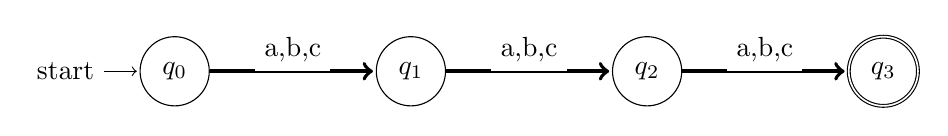
\begin{tikzpicture}[shorten >=1pt,node distance=3cm, on grid, auto]
\node[state,initial] (q_0)	{$q_0$};
\node[state] 		 (q_1) [right=of q_0]	{$q_1$};
\node[state] 		 (q_2) [right=of q_1] {$q_2$};
\node[state, accepting] (q_3) [right=of q_2] {$q_3$};

		\tikzset{every node/.style={fill=white}}
	\tikzset{mystyle/.style={->,double=black}}

\path[->]
	(q_0) edge [mystyle] node {a,b,c} (q_1)
	(q_1) edge [mystyle] node {a,b,c} (q_2)
	(q_2) edge [mystyle] node {a,b,c} (q_3);

\end{tikzpicture}

	

\end{document}